\RequirePackage[2020-02-02]{latexrelease}
\documentclass[letter,scriptaddress,twocolumn, prl]{revtex4}

\usepackage{amsmath}%,amssymb} 
\usepackage{makeidx}
\usepackage{amsfonts}
\usepackage[ansinew]{inputenc}
%\usepackage[usenames,dvipsnames]{pstricks}
%\usepackage{subfigure}
\usepackage{epsfig}
\usepackage{float}
%\usepackage{pst-grad} % For gradients
%\usepackage{pst-plot} % For axes
\usepackage[colorlinks,hyperindex]{hyperref}
\hypersetup
{
colorlinks,%
citecolor=black,%
linkcolor=black,%
urlcolor=black,%
}

\setlength\textheight{24.5cm}

% --- Comandos novos ---
\newcommand{\dket}[1]{\left| #1 \right)}
\newcommand{\E}[1]{\frac{\hbar^2 #1 ^2}{2m_0}}
\newcommand{\dbra}[1]{\left( #1 \right|}
\newcommand{\dsubmin}[1]{\left( #1 \right)}
\newcommand{\dbraket}[2]{\left( #1 | #2 \right)}
\newcommand{\dbraketm}[3]{\left( #1 \left| #2 \right| #3 \right)}
\newcommand{\ket}[1]{\left| #1 \right\rangle}
\newcommand{\bra}[1]{\left\langle #1 \right|}
\newcommand{\submin}[1]{\left\langle #1 \right\rangle}
\newcommand{\braket}[2]{\left\langle #1 \right. \left| #2 \right\rangle}
\newcommand{\braketm}[3]{\langle #1 \mid #2 \mid #3 \rangle}
\newcommand{\pinterno}[2]{\left( #1 , #2 \right)}
\newcommand{\comut}[2]{\left[ #1 , #2 \right]} % THE COMUTATOR
\newcommand{\seitz}[2]{\left\{ \, #1 \mid  #2 \, \right\}}
\newcommand{\rep}{\emph{rep} }
\newcommand{\irep}{\emph{irrep} }
\newcommand{\ordem}[1]{\mid #1 \mid}
\newcommand{\op}[1]{\mathbb #1 }
\newcommand{\group}[1]{\mathcal #1 }
\newcommand{\vet}[1]{\mathbf #1 }
\newcommand{\argu}[1]{\left( #1 \right)}
\newcommand{\kp}{\vet{k}\cdot\vet{p}}

\makeindex

%--------------------------------------------------------
\begin{document}

\title{Computational Simulation of the 2d Ising Model}

\author{Alex Roseman}
\author{Adrian Hall}
\date{\today}

\begin{abstract}

\end{abstract}

\maketitle

\begin{figure*}[t]
	\begin{center}
		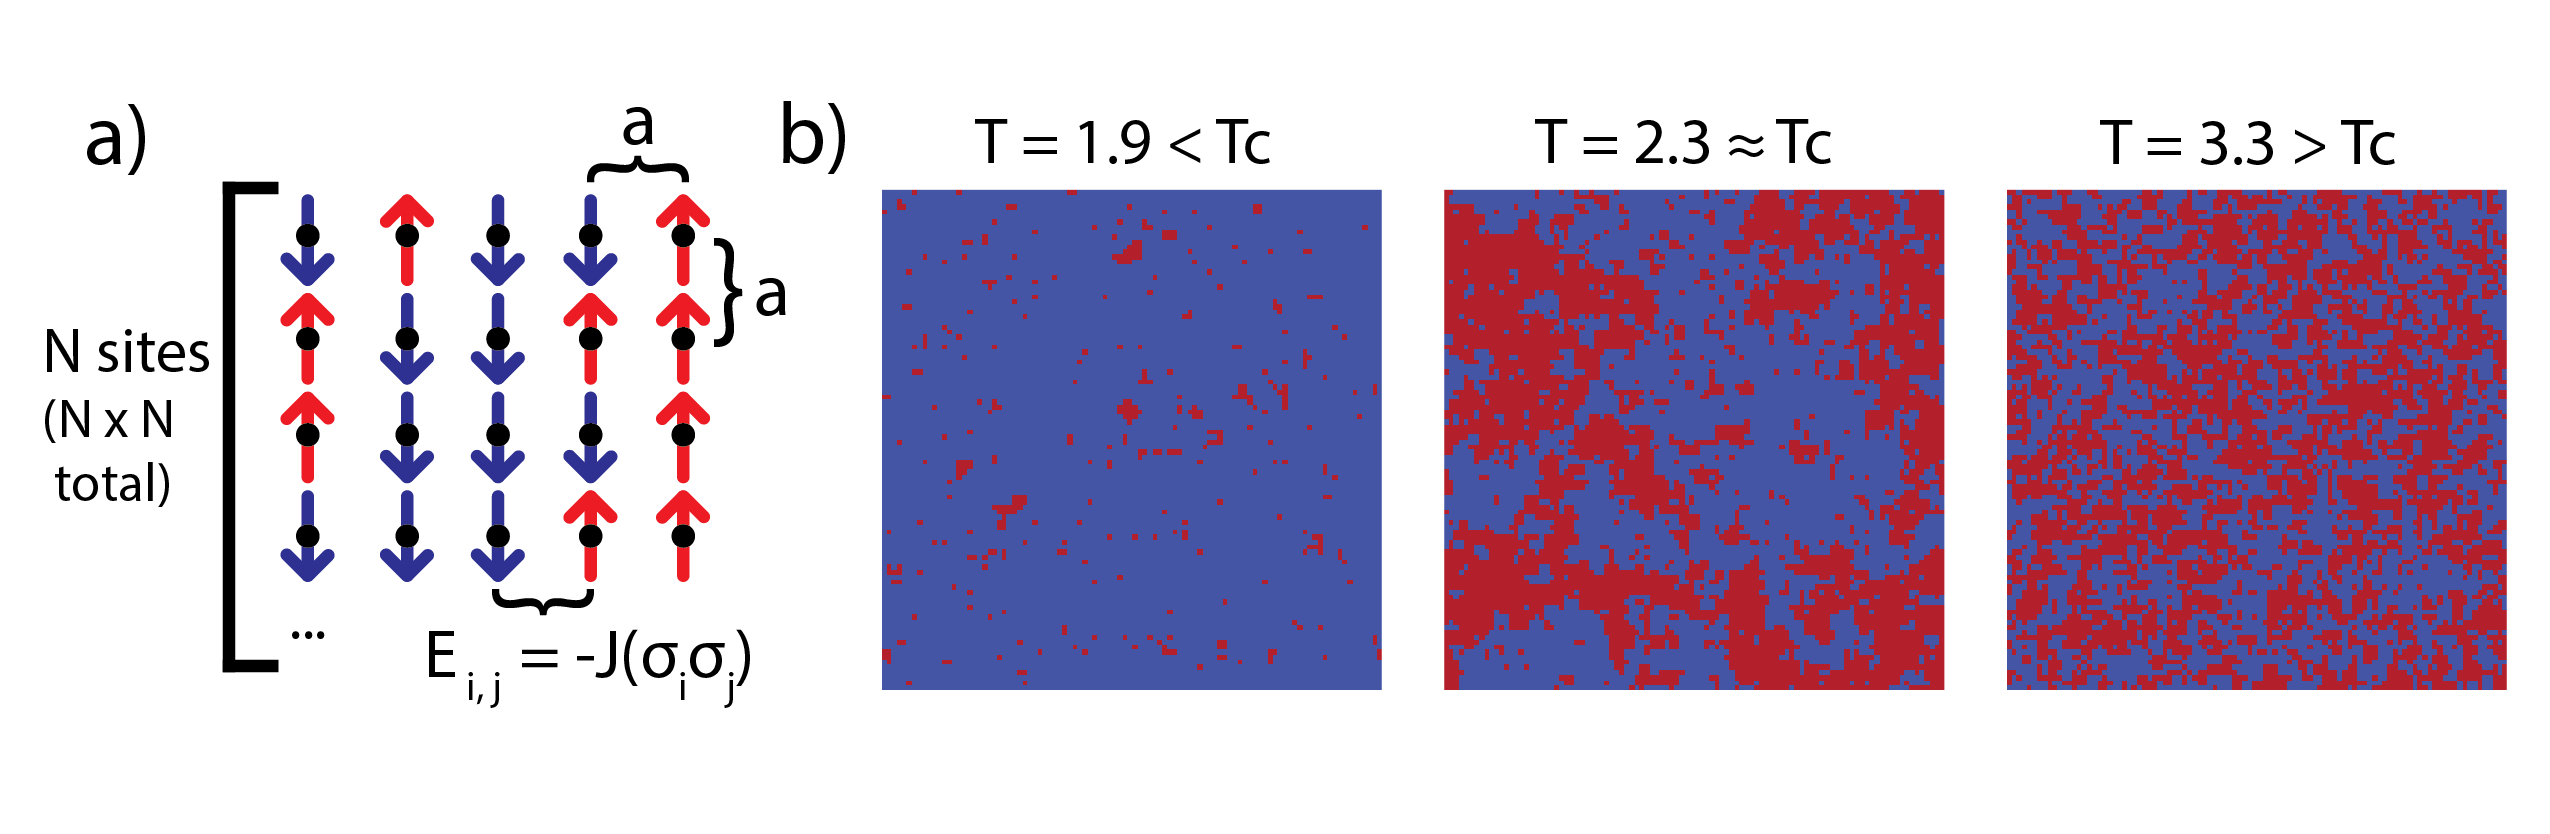
\includegraphics[width=1\textwidth]{figs/fig1.png}
		\caption{a. A diagram of the square lattice. We use lattice size $N = 100$, lattice distance $a = 1$, interaction energy $J = 1$, and spin = $\sigma = \pm 1$ throughout. $E_{i, j}$ is the interaction energy between adjacent spin sites (the lattice wraps around such that each site has 4 neighbors). b. Snapshots after around ten million simulation steps at the given temperature, showing typical states below, near, and above Tc. Red squares have spin up, blue squares spin down.}
		\label{fig:fig1}
	\end{center}
\end{figure*}

\textbf{Introduction:}

\begin{equation}
	\label{eq:hamiltonian}
	H = -J \sum_{\left\langle i, j \right\rangle}\sigma_i\sigma_j - B \sum_i\sigma_i
\end{equation}

\begin{equation}
	\label{eq:Tc}
	T_c = \frac{2}{\ln{(1+\sqrt{2})}} \approx 2.269 (J/k_B)
\end{equation}

\textbf{Methods:}

We simulate the 2d Ising Model on an $N$ by $N$ square lattice using the Metropolis-Hastings algorithm, a Markov chain Monte Carlo method which enables sampling when one knows only relative, rather than absolute, probabilities. The lattice, along with representative lattice configurations above, near, and below critical temperature, is depicted in \autoref{fig:fig1}.

Throughout the experiment, we use a lattice of size N = 100 with periodic boundary conditions, such that the one-hundredth lattice site in a given row or column is considered adjacent to the first. [The decision to use N = 100 is explained during analysis of correlation length $\xi$.]

The Metropolis-Hastings algorithm generates samples from a distribution via a random walk through state space (here, overall lattice configurations), lingering on states for simulation steps proportional to their probabilities. In this experiment, we use Metropolis sampling to sample from the Gibbs distribution, in which the probability of a state with energy E is proportional to $e^{-\frac{E}{k_BT}}$. The specific algorithm we use is as follows.

At each step:
\begin{enumerate}
	\item A percentage of lattice sites (i.e. particles) are selected randomly (throughout this experiment, this parameter was set to $10\%$).
	\item We calculate the overall change in energy from flipping the spin of each selected particle, $\Delta E_i = 2(J\sigma_i(\sum_j\sigma_j) + B\sigma_i)$, where $\sigma_i$ is the flipped spin of the particle, and $\sigma_j$ are the spins of the particle's four neighbors.
	\item The spin at each selected lattice site is or is not flipped depending on $\Delta E_i$ (the calculation is independent for each site):
	\begin{enumerate}
		\item if $\Delta E < 0$, the spin is flipped.
		\item if $\Delta E > 0$, the spin is flipped with probability $e^{-\Delta E_i/(k_BT)}$
	\end{enumerate}
\end{enumerate}

In the limit of large numbers of simulation steps, this algorithm faithfully recreates the Gibbs distribution. With finite simulation time, one must take care that the simulation converges:

Metropolis sampling traverses state space at a finite speed, here determined by flipping at maximum ten percent of all lattice sites at each step. However, the lattice must be initialized to some state, which could have arbitrarily low probability. It takes the simulation some time to leave behind initial conditions and arrive at a representative state. 

This process can be sped up via annealing, starting at a high temperature and magnetic field, and then slowly lowering them to the experimental values. The high temperature adds energy to the lattice, lowering the pull of local minima to allow the lattice to find overall lower-energy states. The initial magnetic field breaks the symmetry between positive and negative spin, pulling the lattice away from configurations with large magnetic domains and towards ultimately lower-energy states. As an example, consider a lattice initialized to be split in half down the middle, with the left half spin up, and the right half spin-down. This state is significantly higher-energy than a lattice of all spin up, but reaching the uniform lattice requires passing through less-probably states. At low temperatures, this may not be possible, or might take an arbitrarily large number of steps. Similarly, with no external field, the two large domains might each grow in some places while ceding ground in others. 

Annealing helps prevent these situations. In our simulations, we anneal from $T = 4 J$ and $B = .5 J$, linearly decreasing $T$ and $B$ to the experimental temperature and zero, respectively, over 3,000 steps. We then wait another 5000 steps of "burn-in time," to allow transients from the extra temperature and field to dissipate. This does introduce artifacts into the simulation data: magnetization $M$ is somewhat more likely to be positive than negative, especially at low temperatures. However, this effect is ultimately irrelevant: we use only the magnitude of $M$.

The other side of convergence is that Metropolis sampling produces data which is locally correlated: the state at each simulation step is similar to the states which precede and follow it. In this experiment, we take data for a total of 200,000 steps (after annealing and burn-in). This decision is explained in Appendix A.

\textbf{Data and Analysis:}

We calculate three quantities during the simulation. The first is expected energy per lattice site

\begin{equation}
	\label{eq:e_average}
	\submin{E} = \frac{J}{N^2}\sum_{i, j = 1}^{N} \sum_{k} \sigma_{i, j} \sigma_k
\end{equation}

where $\sigma_{i, j}$ is the dimensionless spin of the lattice site at row $i$, column $j$, and $\sigma_k$ are the spins of its four neighbors. $\submin{E}$ is a straightforward measure of energy, with the number of lattice sites factored out so as not to scale with lattice size (as we are interested in the $N\rightarrow\infty$ limit). For figures, we use a dimensionless $\submin{E}$, with units of $[J]$.

We calculate a value for $\submin{E}$ over the whole lattice at each simulation step, then extract the mean and standard deviation over the whole simulation at a given temperature (equivalent to an expected value from the Gibbs distribution because the Metropolis-Hastings algorithm spends time in each state proportionate to its probability). In this experiment, we extract the means and standard deviations from one hundred simulation trials, then generate final values for $\submin{E}_T$ by averaging the means from all one hundred simulations at a given temperature together. We use the standard error of this mean to generate uncertainties, considering each simulation a separate measurement.

Similarly, the expected magnetization per lattice site

\begin{equation}
	\label{eq:e_average}
	\submin{M} = \frac{J}{N^2}\sum_{i, j = 1}^{N} \sigma_{i, j}
\end{equation}

[[the final directly-calculated quantity is...]]

\begin{figure}[h]
	\begin{center}
		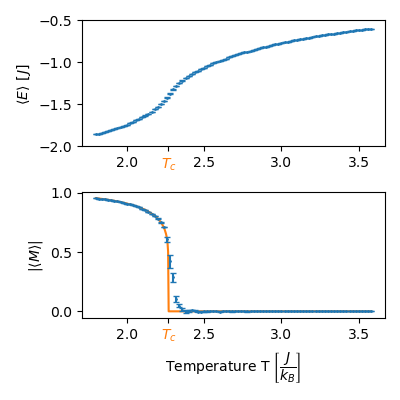
\includegraphics[width=.5\textwidth]{figs/fig2_EMplots.png}
		\caption{Mean energy (top) and absolute magnetization (bottom) per lattice site as computed by MCMC simulation at a range of temperatures. Data is drawn from 97 independent simulations: each data point is the average value of $\left\langle M \right\rangle$ over all simulations; each standard error is the standard error of the mean of $\left\langle M \right\rangle$ over all simulations, treating each $\left\langle M \right\rangle$ as an independent measurement. Analytic Tc (red) and analytic curves (green) plotted for comparison. At first glance, our system appears to reach phase transition at lower temperature than the analytic $T_c$.}
		\label{fig:fig2}
	\end{center}
\end{figure}



\begin{figure}[h]
	\begin{center}
		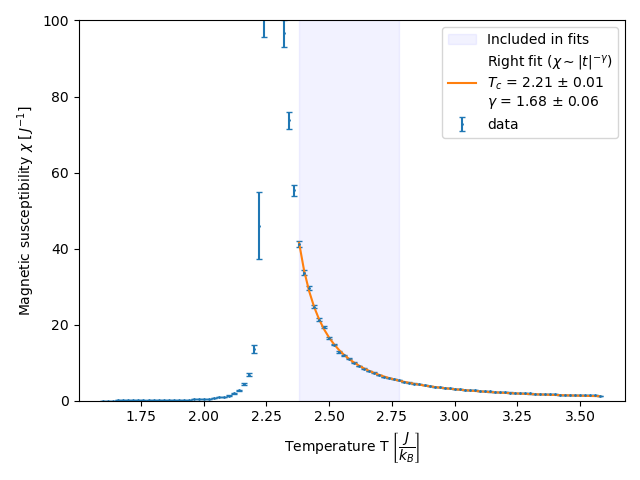
\includegraphics[width=.4\textwidth]{figs/fig3_chi.png}
		\caption{Magnetic susceptibility at a range of temperatures. Susceptibility is calculated from variance in M over each simulation, which is taken as a single measurement. Data points on this graph are the mean of variance(M) over all 97 simulations at a given temperature, and error bars on this graph are the standard error of this mean. Shown in orange is a power law fit with $T_c$ and $\gamma$ considered as free variables, using only the data in the shaded column. NOTE: we intend to merge figures 3 and 4 into a single figure with 2 graphs.}
		\label{fig:fig3a}
	\end{center}
\end{figure}
\begin{figure}[h]
	\begin{center}
		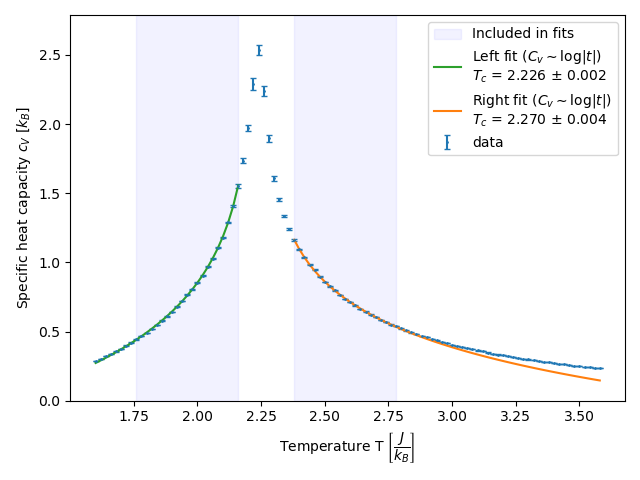
\includegraphics[width=.4\textwidth]{figs/fig3_cv.png}
		\caption{Specific heat at a range of temperatures. Like susceptibility, specific heat is calculated from variance in E across MCMC steps. Data points on this graph are the mean of variance(E) over all 97 independent simulations at a given temperature, and error bars on this graph are the standard error of this mean. Shown in orange and green are logarithmic fits in which $T_c$ was considered a free variable, using only the data in the shaded columns. We generated separate fits on the left and right of Tc. Although the power law should be symmetric, we find significantly different results for Tc. NOTE: we intend to merge figures 3 and 4 into a single figure with 2 graphs.}
		\label{fig:fig3b}
	\end{center}
\end{figure}
\begin{figure}[h]
	\begin{center}
		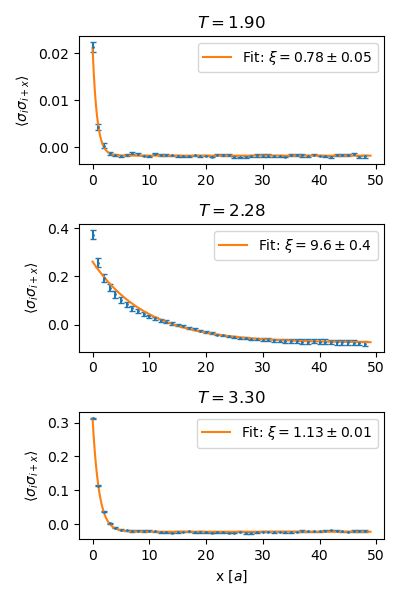
\includegraphics[width=.4\textwidth]{figs/fig4_autocors.png}
		\caption{Autocorrelation functions at representative temperatures: below, near, and above $T_c$. Shown in orange are exponential decay functions fit by least-squares regression to the positive portion of the autocorrelation data, with length scale parameter $\xi$. Autocorrelation seems to become negative (i.e. anticorrelated) after sufficient lattice distance, leading the exponential fit to deviate significantly from the data. This likely plays a role in our terrible estimate for $\nu$. Note: we intend to merge Figs. 5 and 6.}
		\label{fig:fig4a}
	\end{center}
\end{figure}
\begin{figure}[h]
	\begin{center}
		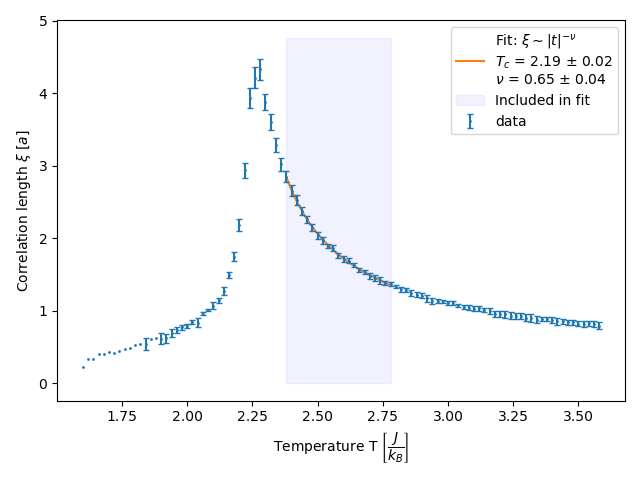
\includegraphics[width=.4\textwidth]{figs/fig4_xi.png}
		\caption{Correlation length $\xi$ at a range of temperatures. These data points are drawn from the fits depicted in Fig. 5, with all the inaccuracy that entails. Uncertainties are drawn from Scipy's curve fit covariance matrix. We intend to include a complete description of the nature of these uncertainties in the body of our report. As with $\chi$ and $c_v$, we fit a power law function (orange) to the data in the shaded region, with $T_c$ and $\nu$ as free parameters. Note: we intend to merge Figs. 5 and 6.}
		\label{fig:fig4b}
	\end{center}
\end{figure}
\begin{figure*}[h]
	\begin{center}
		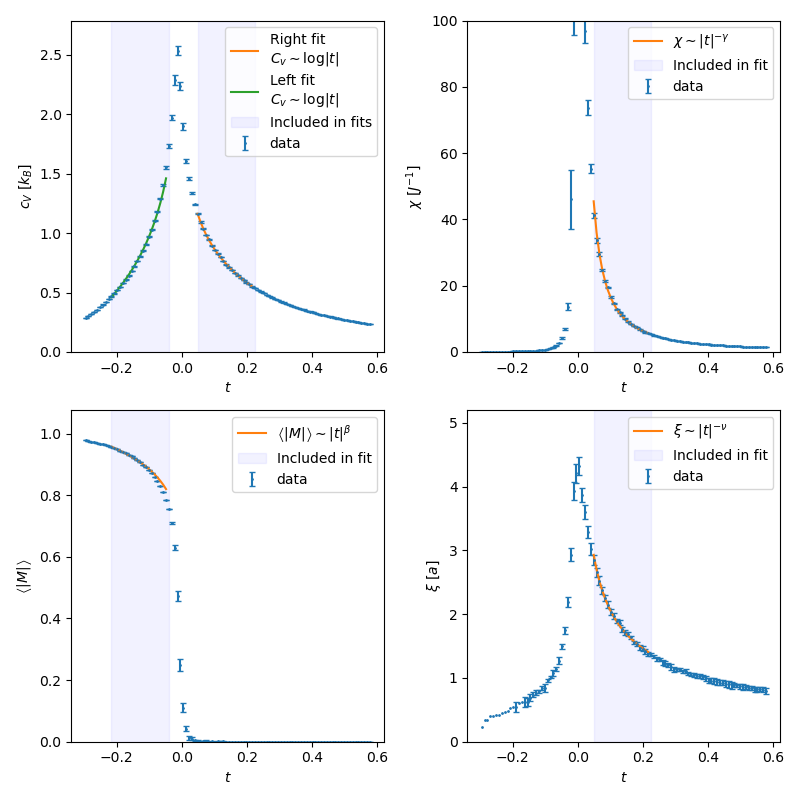
\includegraphics[width=1\textwidth]{figs/fig5_crit_exponents.png}
		\caption{Power law fits for the critical exponents for $c_V$ ($\alpha$) (upper left), $\chi$ ($\gamma$) (upper right), $|M|$ ($\beta$) (lower left), and $\xi$ ($\nu$) (lower right). We attempt to show $\alpha = 0$ by successfully fitting a logarithmic function to $c_V$. In each graph, the x-axis is the normalized temperature $t = \frac{T - T_c}{T_c}$, where $T_c$ is the analytic value of $T_c$. As before, only data from the shaded regions was used for fits. We find the following values: $\gamma = 1.40 \pm .01$, $\beta = 0.103 \pm .002$, $\nu = 0.49 \pm .01$. All critical exponents are, of course, unitless. We have not checked identities because these values are clearly broken, $\nu$ especially (see abstract for details).}
		\label{fig:fig5}
	\end{center}
\end{figure*}

\textbf{Acknowledgements:}
	Prof. Navon, Prof. Newburgh, HongJoon

\bibliographystyle{unsrt} 
%\bibliography{/home/thiago/bibtex/articles,/home/thiago/bibtex/books}

\begin{thebibliography}{}
	
	\bibitem{Onsager}
	Lars Onsager,
	\textit{Crystal Statistics. I. A Two-Dimensional Model with an Order-Disorder Transition},
	Physical Review {\bf 65}, 117 (1944).
	
	
\end{thebibliography}

\appendix
\section{Appendix A: Convergence}

\begin{figure}[h]
	\begin{center}
		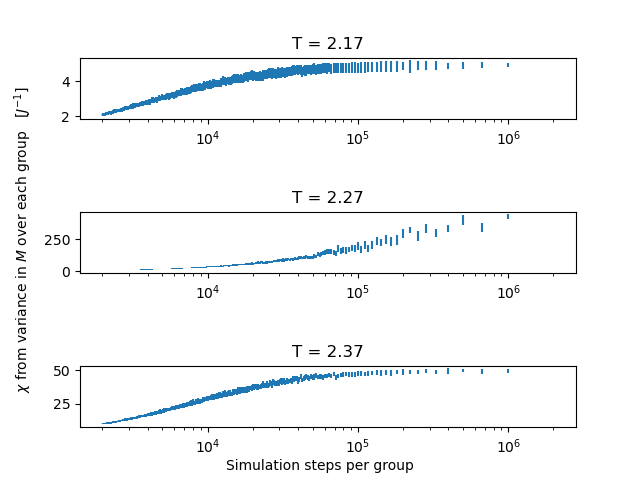
\includegraphics[width=.4\textwidth]{figs/figA1.png}
		\caption{$\chi$ values calculated with data from a simulation of 2,000,000 analyze steps. The total 2,000,000 steps were split as evenly as possible into groups of $n_{steps}$ (x axis), and variance in M was calculated across each group. Each data point is the average variance over all such groups.}
		\label{fig:figA1}
	\end{center}
\end{figure}

\end{document}
